\documentclass{standalone}
\usepackage{tikz}
\usepackage{standalone}
\usetikzlibrary{calc}

\begin{document}
    \begin{tikzpicture}
        \node[chain] (layer) {\footnotesize{\textbf{LSTM}}};
        \node[input, font=\boldmath]  (i) at ($(layer)+(0, -2.15)$) {$\mathbf{x_t}$};
        \node[above=1cm of layer,output, font=\boldmath] (o) {$\hat{y}_t$};

        \draw (layer) edge[->, out=90, in=-90, thick, orange] (o);
        \draw (i) edge[->, out=90, in=-90, thick, orange] (layer);

        \path (layer.west) ++ (-1em,2em) coordinate (aux);
        \draw[thick,-latex,rounded corners, orange] (layer.east) -| ++ (1em,2em) -- (aux)
        |- (layer.west);

        \node[right=1cm of layer] (eq) {$=$};

        \node[right=2cm of layer, chain, orange!20] (layer1) {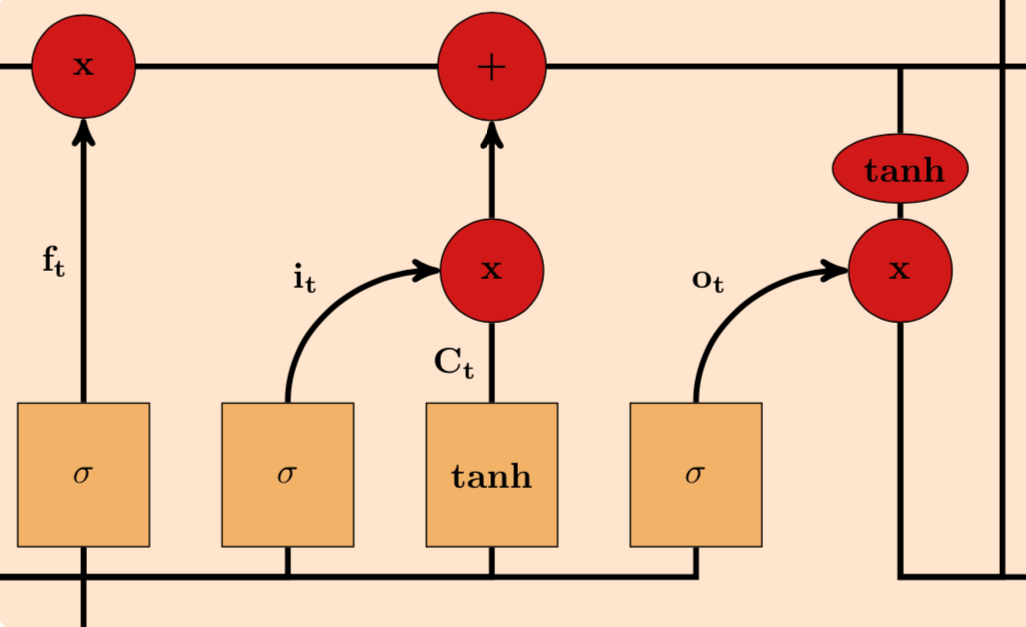
\includegraphics[width=\textwidth]{src/chapters/07/img/cell}};
        \node[input, font=\boldmath]  (i1) at ($(layer1)+(-.88, -2.15)$) {$x_1$};
        \node[output, font=\boldmath] (o1) at ($(layer1)+(1.005, 2.25)$) {$\hat{y}_1$};
        \draw [<-, thick, black] (o1) -- ++ (0, -1.46);
        \draw [->, thick, black] (i1) -- ++ (0, 1.4);

        \node[right=1cm of layer1, chain, orange!20] (layer2) {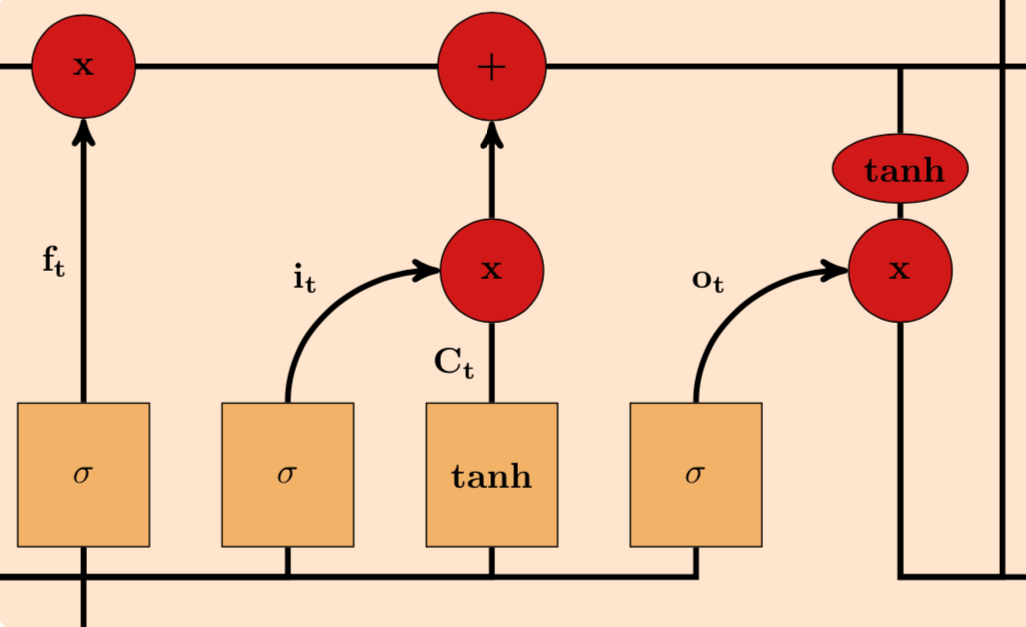
\includegraphics[width=\textwidth]{src/chapters/07/img/cell}};
        \node[input, font=\boldmath]  (i2) at ($(layer2)+(-.88, -2.15)$) {$\mathbf{x_2}$};
        \node[output, font=\boldmath] (o2) at ($(layer2)+(1.005, 2.25)$) {$\hat{y}_2$};
        \draw [<-, thick, black] (o2) -- ++ (0, -1.46);
        \draw [->, thick, black] (i2) -- ++ (0, 1.4);

        \node[right=1cm of layer2] (dots) {\Huge{$\dots$}};

        \node[right=.5cm of dots, chain, minimum width=7em, orange!20] (layer4) {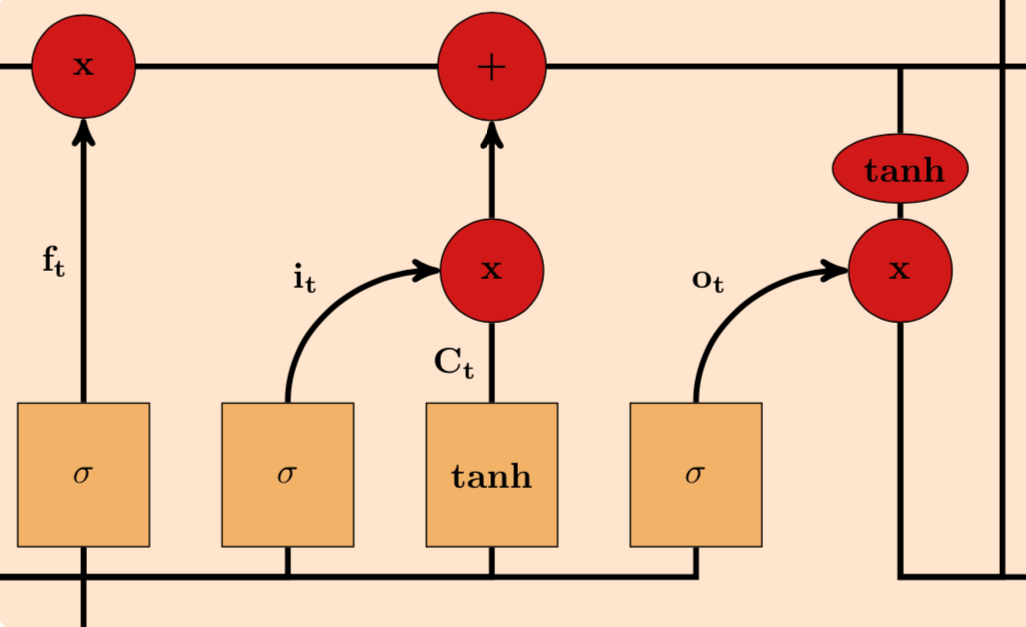
\includegraphics[width=\textwidth]{src/chapters/07/img/cell}};
        \node[input, font=\boldmath]  (i4) at ($(layer4)+(-.88, -2.15)$) {$\mathbf{x_t}$};
        \node[output, font=\boldmath] (o4) at ($(layer4)+(1.005, 2.25)$) {$\hat{y}_t$};
        \draw [<-, thick, black] (o4) -- ++ (0, -1.46);
        \draw [->, thick, black] (i4) -- ++ (0, 1.4);

        \draw [->, thick, black] (layer1) ++ (1.2, .505) node[above right] {\tiny$C_1$} -- (6.6, .505);
        \draw [->, thick, black] (layer1) ++ (1.2, -.545) node[below right] {\tiny$h_1$} -- (6.6, -.545);

        \draw [->, thick, black] (layer2) ++ (1.2, .505) node[above right] {\tiny$C_2$} -- (10, .505);
        \draw [->, thick, black] (layer2) ++ (1.2, -.545) node[below right] {\tiny$h_2$} -- (10, -.545);

        \draw [->, thick, black] (dots) ++ (.5, .505) node[above right] {\tiny$C_t$} -- (11.8, .505);
        \draw [->, thick, black] (dots) ++ (.5, -.545) node[below right] {\tiny$h_t$} -- (11.8, -.545);
    \end{tikzpicture}
\end{document}